
\chapter{The HPS Apparatus}

\section{Introduction}

The HPS experiment engineering run was conducted in the Spring of 2015 at the 
Thomas Jefferson National Accelerator Facility (JLab) in Newport News, VA 
within experimental Hall B.  HPS utilized CEBAF's high luminosity electron beam,
operating at an energy of 1.056 GeV and current of 50 nA, incident on a thin
(~0.125\% $X_{0}$) tungsten target to search for an $A'$ with a mass in the 
range of 20 - 100 MeV.  Sensitivity to such a search requires the precision 
measurement of both the invariant mass and vertex of the $A'$.  This is 
achieved by placing a silicon vertex tracker (SVT) immediately downstream 
(10 cm) from the target inside of an analyzing magnet and using an 
electromagnetic calorimeter to trigger.

At this energy, the decay products of the electroproduced $A'$ are highly 
boosted. As a result, obtaining the complete kinematic information required
to reconstruct the $A'$ necessitates 
the need to place the detector in close proximity to the intense primary beam
plane.  The distance of the detector from the beam plane is limited by a 
``dead zone'' occupied Coulomb scattered electrons and radiative secondaries. 
Maximizing the sensitivity to a low mass $A'$, therefore, requires minimizing
the size of the dead zone.

The chapter that follows, a detailed description of the HPS apparatus will
be given.

\section{CEBAF}

The electrons injected into the accelerator were a result of photoemission from
a superlattice photocathode.  The photoemission electrons are released into an
extremely high vacuum environment at a pressure of $10^{-11}$ to $10^{-12}$ 
Torr.  The free electrons are then delivered into the injector by a 100 keV 
electron gun.  The injector itself then accelerates the electron bunches to 
an energy of 67 MeV by 2 1/4 cryomodules before being delivered into the 
accelerator.  

% Need to add a sentence explain why we ran as a 6 GeV era detector
The CEBAF accelerator is composed of two linacs arranged in a racetrack
configuration as shown on Fig \ref{fig:cebaf}. Each of the linacs consist
\begin{figure}[h]
    \centering
    \caption{The Continous Electron Beam Accelerator Facility.}
    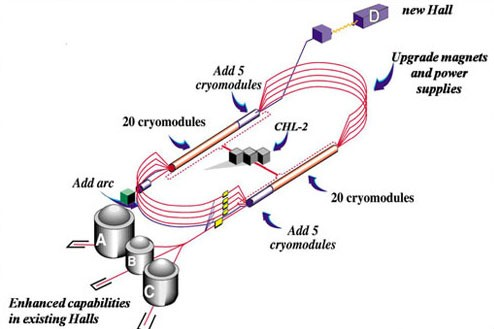
\includegraphics[width=0.5\textwidth]{images/cebaf.jpg}
    \label{fig:cebaf}
\end{figure}
of () cryomodules which is capable of accelerating the electron bunches 
by () GeV per pass up to a maximum of () passes per linac.  The number of 
passes depends on the energy requirements of the experiment taking place.
The electron bunches are delivered to each experimental hall by an RF seperator
operating at a frequency of 499 MHz. 

The acceleration of the electron beam takes place using a 5-cell 
superconducting radio frequency (SRF) cavities made of ultra-pure Niobium 
operating at 1497 MHz.  Two of the SRF cavities are joined and placed in a 
sealed helium container forming a cryounit.  () cryounits are joined in an
insulating vacuum environment to for a cryomodule.  The cryomodules also
contain the necessary instrumentation both to power the SRF cavities and keep
them at an operating temperature of 2 K.

\section{Beam Line}

\section*{Silicon Vertex Tracker}

\subsection*{Layout}

The SVT is comprised of six measurement layers, each consisting of a pair of
closely-spaced silicon planes as shown in Fig. \ref{fig:svt_layout_render}.
\begin{figure}[h]
    \centering
    \caption{A render of the Silicon Vertex Tracker.}
    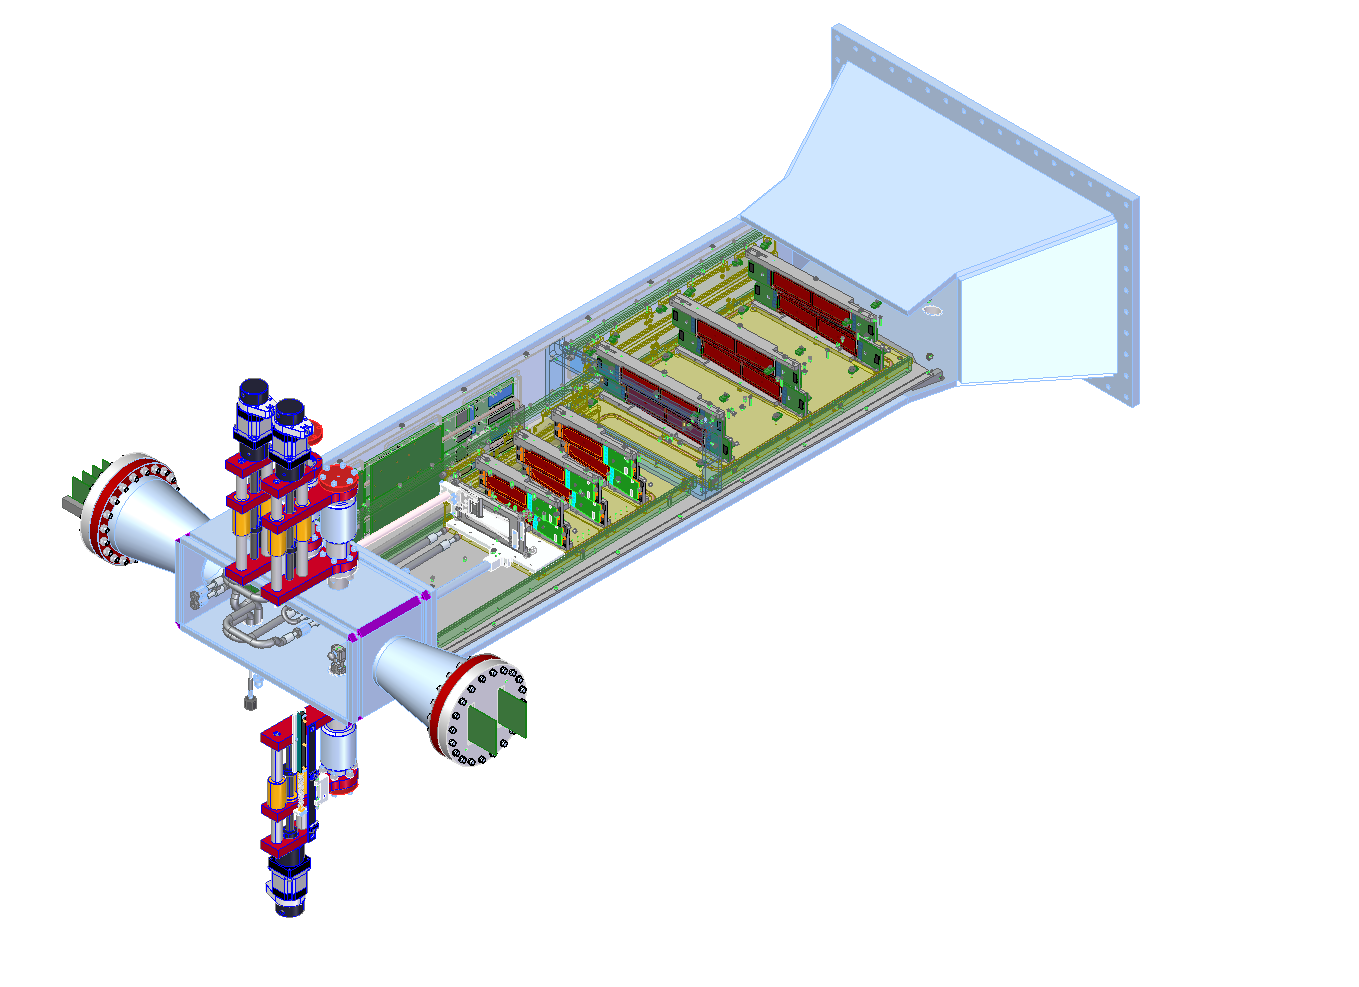
\includegraphics[width=0.5\textwidth]{images/svt_layout_render.png}
    \label{fig:svt_layout_render}
\end{figure}
A stereo angle is introduced between the two planes within each layer allowing
for the measurement of both the vertical and bend coordinate of a hit, in turn, 
enabling full 3D hit reconstruction.  The first three layers consist of a
% needs a sentence explaning why 100 mrad stereo was used.  According to the
% proposal, it balances acceptance against vertexing resolution.
single sensor and use a stereo angle of 100 mrad. In order to better match the
acceptance of the ECal, the coverage of the last three layers is two sensors 
% Insert a sentence explaining why 50 mrad? According to the proposal it's too
% cut down the number of bad tracks created from ghost hits due to layers with
% the same stereo angle.
% Why use a sixth layer? I guess it's not that important but should be in here
% nontheless
wide and use a stereo angle of 50 mrad.  In total, the SVT makes use of 36
sensors, which amounts to 23,004 channels.  The SVT layout is summarized in 
Table \ref{tab:svt_layout}.

%%%%%%%%%%%%%%%%%%%%%%%%%%%
%%% Table of SVT layout %%%
%%%%%%%%%%%%%%%%%%%%%%%%%%%
\begin{table}[t]
 \begin{center}
\begin{tabular}{l|cccccc}  
Layer & 1 & 2 & 3 & 4 & 5 & 6 \\ \hline
$z$ position from target [cm]    & 10 & 20 & 30 & 50 & 70 & 90 \\
Stereo angle [mrad] & 100 & 100 & 100 & 50 & 50 & 50 \\
Bend plane resolution [$\mu$m] & $\approx$6 & $\approx$6 & $\approx$6
& $\approx$6 & $\approx$6 & $\approx$6 \\
Non-bend plane resolution [$\mu$m] & $\approx60$ & $\approx60$ & $\approx60$
& $\approx120$ & $\approx120$ & $\approx120$ \\
\hline
\end{tabular}
\caption{The proposed layout of the SVT.}
\label{tab:svt_layout}
\end{center}
\end{table}
%%%%%%%%%%%%%%%%%%%%%%%%%%%



The SVT is split into upper and lower tracking volumes in order to avoid
the 15 mrad ``dead zone'', putting the active area of the sensors at 1.5 mm
from the beam plane.  The layers are mounted on upper and lower support 
structures that are hinged on the downstream end of the SVT.  This allows
adjustment of the vertical position of the sensors remotely by a motion
control system, in response to experimental conditions.

\subsection*{Sensors}

At the energies at which HPS will operate, the uncertainty of both the mass and
vertex is dominated by multiple Coulomb scattering.  As a result, 
the material budget of the SVT must be minimized in order to achieve the 
optimal mass and vertex resolutions.  Furthermore, the necessity of placing the
SVT in close proximity to the beam requires a sensor technology that is 
radiation tolerate.  With these considerations in mind, silicon microstrip 
sensors were chosen.

The SVT used used $p^{+}$ on $n$-bulk, single sided, AC-coupled, 
polysilicon-biased sensors manufactured by Hamamatsu Photonics
corporation on <100> silicon for the cancelled Run IIb D0 run.
The sensors are 320 $\mu$m thick and have 
a sense (readout) pitch of 30 (60) $\mu$m. All sensors were qualified to 
1 kV and can tolerate a dose of 1.5 $\times 10^{14}$ 1 MeV neq/cm$^{2}$.  The 
sensor specifications are listed on Table \ref{tab:sensor_specs}

\begin{table}[t]
    \begin{center}
        \begin{tabular}{rc}
            Cut Dimensions & 100 mm x 40.34 mm \\
            Active Area & 98.33 mm x 38.34 mm \\
            Readout (Sense) pitch & 60 (30) $\mu$m \\
            # Readout (Sense) strips & 639 (1277) \\
            Depletion Voltage & 40 V - 300 V \\
        \end{tabular}
        \caption{Sensor specs.}
        \label{tab:sensor_specs}
    \end{center}
\end{table}

\subsection*{Readout}

The sensor are continously read out using the APV25 readout chip developed for
the Compact Muon Solenoid detector at the Large Hadron Collider.  The APV25
consist of 128 channels of a pre-amplifier coupled to a shaping amplifier. The
shaper signal is sampled at 41.6 MHz into an analog pipeline 192 cells deep.
At the nominal operating points, the shaping time is equal to 50 ns and the
expected noise performance is ...  During the engineering run, the APV25's
were operated in multi-peak mode, with six samples being read out per 
trigger.  The six samples were then used to extract the $t0$ and amplitude 
of the signal.  A summary of the specifications of the AVP25 is shown
on Table ().

\subsection*{Modules}

\section{Electromagnetic Calorimeter}

\subsection{Layout}

\section{Trigger and Data Acquisition}

